\documentclass{article}%
\usepackage[T1]{fontenc}%
\usepackage[utf8]{inputenc}%
\usepackage{lmodern}%
\usepackage{textcomp}%
\usepackage{lastpage}%
\usepackage[head=40pt,margin=0.5in,bottom=0.6in]{geometry}%
\usepackage{graphicx}%
%
\title{\textbf{Lorent Saleh se reunió con Bachelet para denunciar violaciones de DD HH}}%
\author{EL NACIONAL WEB}%
\date{06/12/2018}%
%
\begin{document}%
\normalsize%
\maketitle%
\textbf{URL: }%
http://www.el{-}nacional.com/noticias/politica/lorent{-}saleh{-}reunio{-}con{-}bachelet{-}para{-}denunciar{-}violaciones\_262365\newline%
%
\textbf{Periodico: }%
EN, %
ID: %
262365, %
Seccion: %
Política\newline%
%
\textbf{Palabras Claves: }%
Política, Gobierno\newline%
%
\textbf{Derecho: }%
1.2%
, Otros Derechos: %
18%
, Sub Derechos: %
1.2.2%
\newline%
%
\textbf{EP: }%
NO\newline%
\newline%
%
\textbf{\textit{El ex preso político pidió a la alta comisionada de Derechos Humanos de la ONU que realice una visita objetiva a Venezuela}}%
\newline%
\newline%
%
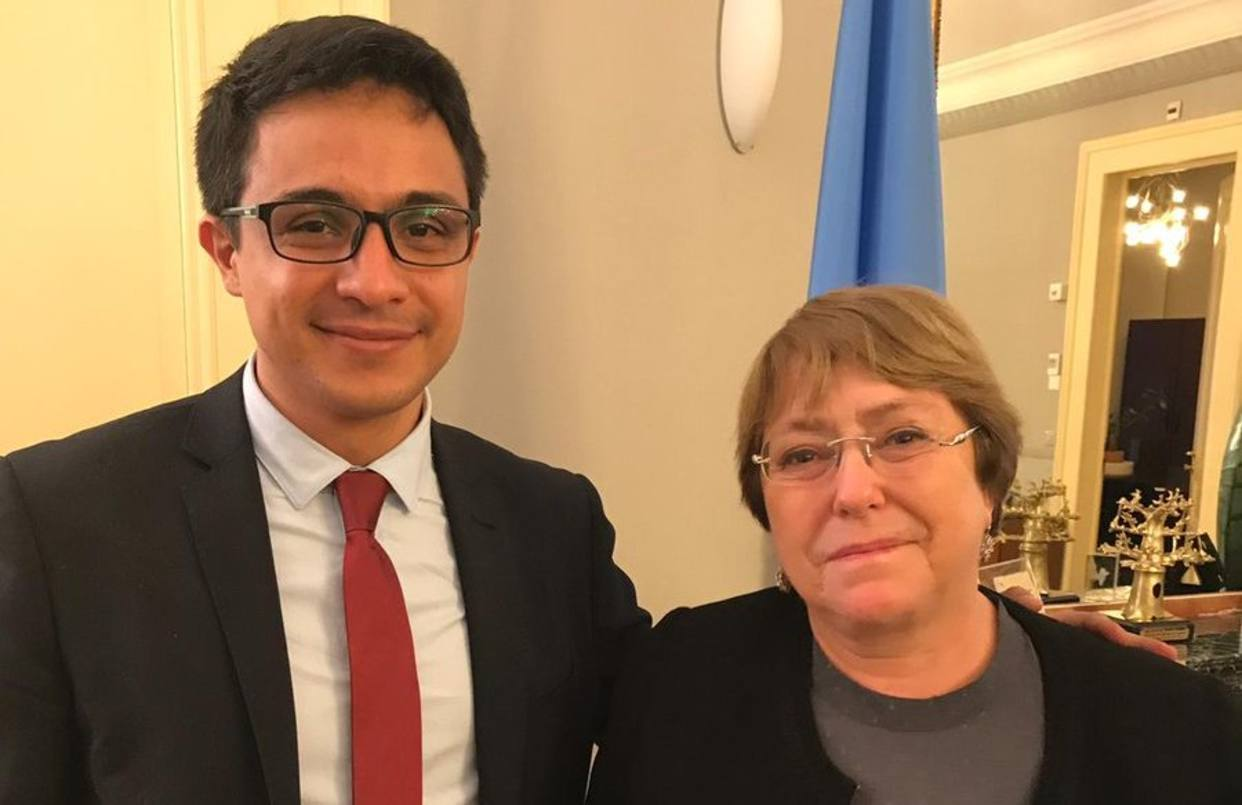
\includegraphics[width=300px]{148.jpg}%
\newline%
%
Lorent Saleh, activista venezolano de derechos humanos~exiliado en Madrid, se reunió este jueves con Michelle Bachelet, alta comisionada de Derechos Humanos de la ONU, para denunciar y relatar su testimonio como preso político en Venezuela.%
\newline%
%
"Además de exponer las graves violaciones a los DD HH que se aplican sistemáticamente en nuestro país, manifestamos la necesidad de que se dé una visita que cumpla rigurosamente las pautas de objetividad para que no sea objeto de oscuras manipulaciones por quienes usurpan el poder", escribió Saleh en Twitter.%
\newline%
%
Destacó que la crisis que atraviesa el país llamó la atención del organismo internacional por lo que pidió seguir cultivando y alimentando las denuncias a instancias de la ONU.%
\newline%
%
\end{document}